\documentclass[12 pt]{book}
\usepackage{amsmath}
\usepackage{amsthm}
\usepackage[paperwidth=5 in,paperheight=5 in,left=7 mm, right=7 mm, top=15 mm, bottom=16 mm]{geometry}
\usepackage{graphics}
\usepackage{fontawesome}
\usepackage{enumitem}
\usepackage{marvosym}
\newcommand{\myitem}{\refstepcounter{enumi}\item[$^\star$\theenumi.]}
\newcommand{\mmyitem}{\refstepcounter{enumi}\item[$^{\star \star}$\theenumi.]}
\setcounter{page}{01}

\usepackage[utf8]{inputenc}
\usepackage{xcolor}
\setlength{\arrayrulewidth}{0.1 mm}
%BLUE%
%\definecolor{Mycolor2}{HTML}{3D9BE9}
\definecolor{Mycolor2}{HTML}{33cccc}
%\definecolor{Mycolor2}{HTML}{000000}

%%----HEADER &&& FOOTER----%%

\usepackage{fancyhdr}


\pagestyle{fancy}
\fancyhf{}
\setlength{\headheight}{8 mm}
%\fancyhead[CE,CO]{ \Times\Large{\textbf{\textls*[100]{\textcolor{tomato}{\textit{Illustration}}}}}}

\fancyhead[CE,CO]{\Large{\textbf{\textls*[250]{\textcolor{tomato}{SOLVE ME! \\[-5 mm]{\Large{\textbf{\textls*[5000]{\textcolor{black}{\scalebox{.42}{ROTATION}}}}}}     }}}}}

%\fancyfoot[CE,CO]{\Large{\textls*[10]{\textcolor{tomato}{\Times\textit{\tikz \draw [-{Stealth[red]}, line width=4.5,line cap=round] (0,0) node[below=-13.5 mm,scale=2.2,below left]{\textbf{Solution}}--(1.65,0);}}}}}

\renewcommand{\headrulewidth}{0 mm}
\renewcommand{\footrulewidth}{0 mm}


\DeclareMathOperator{\Ln}{ln}

%%----FONT &&& MATHS_FONT----%%

\usepackage{amssymb}
\usepackage{upgreek,xspace}
\newcommand*{\rom}[1]{\expandafter\@\romannumeral #1}


\usepackage[utopia]{mathdesign}
\renewcommand{\familydefault}{\sfdefault}
\usepackage[scaled=1]{helvet}
\newcommand*\Times{\fontfamily{ptm}\selectfont}

%%%------PACAKAGES------%%%

\usepackage[letterspace=120]{microtype}
\usepackage{enumitem}
\usepackage{multicol}
\usepackage{pgfplots}
\pgfplotsset{width=8cm,compat=1.16}
\usepackage{tikz}
\usepgfplotslibrary{fillbetween}
\usetikzlibrary{quotes,angles,patterns,through,calc}
\usepgflibrary{arrows.meta}
\usetikzlibrary{decorations.pathmorphing}
\usetikzlibrary{decorations.markings}
\usetikzlibrary{arrows.meta,bending}
\usepackage{rotating}
\usepackage{tikz-3dplot}
\include{tikz-3dplot}
\usepackage[american voltages, american currents,siunitx]{circuitikz}
\usepackage{circuitikz}
\usetikzlibrary{fit,positioning}
\usetikzlibrary{optics}
\usetikzlibrary{intersections}
\usetikzlibrary{decorations.pathreplacing}
\usepgflibrary{decorations.shapes}
\usepackage{setspace}
\setstretch{1.1}
\usepackage{tkz-tab} [3]
\usepgflibrary{fadings}
%\ctikzset{bipoles/cuteinductor/coils=6}
\usetikzlibrary{decorations.pathmorphing,patterns}


\usepackage{vwcol}[widths={0.25,0.75}]


\usepackage{color}
\usepackage[autostyle]{csquotes}


\usepackage{xcolor}
\definecolor{Mycolor2}{HTML}{33cccc}
\definecolor{One}{HTML}{336666}
\definecolor{Two}{HTML}{666666}
\definecolor{Three}{HTML}{cc6699}


%  black--brown--black %
\definecolor{Four}{HTML}{000000}
\definecolor{Five}{HTML}{330000}
\definecolor{Six}{HTML}{000000}

\definecolor{Seven}{HTML}{ff6666}
\definecolor{Eight}{HTML}{330066}
\definecolor{Nine}{HTML}{cc3333}
\definecolor{tomato}{HTML}{FF6347}
\definecolor{darkblue}{HTML}{2c3e50}
\definecolor{blackm}{HTML}{363636}
\definecolor{pink}{HTML}{ff6666}





\tikzset{
bigger/.style={decoration={shape start size=.25cm, shape end size=1cm}}, smaller/.style={decoration={shape start size=1cm, shape end size=.25cm}}, decoration={shape backgrounds,
shape sep={.25cm, between borders},shape scaled}
}





 % \tikzset{every to/.style={append after command={[draw,dashed]}}}




\def\spring[#1]#2(#3)#4 to (#5)% [draw options] (center) (initial angle:final angle:radius)
  {\draw[#1,line cap=round] (#3)--($(#3)+({0.5},{0})$) ($(#5)-({0.5},{0})$)--(#5);
  	\draw[#1,decoration={aspect=0.3, segment length=1.7 mm, amplitude=3 mm,coil}, decorate]($(#3)+({0.5},{0})$)--($(#5)-({0.5},{0})$);
  }



\tikzset{
  mirror->/.style={postaction={decorate,black!95,draw,thick,
decoration={border,amplitude=-0.25cm,angle=45,segment length=0.22cm,pre length=0.5 mm}}
  }
}



\def\centerarc[#1]#2(#3)#4(#5:#6:#7)% [draw options] (center) (initial angle:final angle:radius)
  {\draw[#1]($(#3)+({#7*cos(#5)},{#7*sin(#5)})$)arc(#5:#6:#7);}



\newcommand{\sm}{\begin{minipage}[c]{0.1\linewidth}
{\Huge{\textcolor{tomato}{\textbf{ }}}}
\end{minipage}}

\newcommand{\AxisRotator}[1][rotate=0]{%
    \tikz [x=0.25cm,y=0.60cm,line width=.2ex,-stealth,#1] \draw (0,0) arc (-120:120:1 and 1);%
}


%%%%%%       Problem Number        %%%%%%%%
%%%%%%       Problem Number        %%%%%%%%

\newcommand{\nm}{\begin{minipage}[c]{0.1\linewidth}
{\Huge{\textcolor{tomato}{\textbf{21. }}}}
\end{minipage}}

%%%%%%       Problem Number        %%%%%%%%
%%%%%%       Problem Number        %%%%%%%%

\newcommand{\vl}{{{\textcolor{tomato}{\textbf{\vrule width 2.25 pt{}}}}}}

\newenvironment{question}
{	
	\nm  \vl \,
	\begin{minipage}[l]{0.86\linewidth}
	\begin{itshape}
	\large\Times\textit{}
}
{
	\end{itshape}
	\end{minipage}
}


\newenvironment{options}
{	
	\sm ~
	\begin{minipage}[l]{0.86\linewidth}
	\begin{multicols}{2}
	\begin{enumerate}[label={(\roman*)}, itemsep=4 mm]
	\normalsize{}
}
{
	\end{enumerate}
	\end{multicols}
	\end{minipage}
}


\newenvironment{v-options}
{	
	\sm ~
	\begin{minipage}[l]{0.86\linewidth}
	\begin{enumerate}[label={(\roman*)}, itemsep=4 mm]
	\normalsize{}
}
{
	\end{enumerate}
	\end{minipage}
}



\newenvironment{definition}
{
	\begin{center}
	\begin{itshape}
	\normalsize\Times\textit{}
}
{
	\end{itshape}
	\end{center}
}


\newenvironment{note}
{
	\begin{center}
	\begin{itshape}
	\normalsize\Times\textit{}
}
{
	\end{itshape}
	\end{center}
}


\newenvironment{calculations}
{
	\begin{itshape}
	\normalsize\Times\textit{}
}
{
	\end{itshape}
}


\newenvironment{q-options}
{	
	\sm ~
	\begin{minipage}[l]{0.86\linewidth}
	\begin{note}
	\begin{enumerate}[label={(\roman*)}, itemsep=1 mm]
	\normalsize{}
}
{
	\end{enumerate}
	\end{note}
	\end{minipage}
}



\newcommand{\physics}{\normalsize{\textcolor{tomato}{\textls*[100]{{\hspace*{75 mm} @10xphysics}}}}}
\newcommand{\solution}{\centering\Large\Times\textbf{\textcolor{tomato}{\textls*[100]{ \textit{\\[-20 mm]Solution}}} }}
\newcommand{\calculation}{\centering\large\Times{\textcolor{tomato}{ \textit{\\[-18 mm]calculations:\\}} }}
\newcommand{\integration}{\centering\large\Times{\textcolor{tomato}{ \textit{\\[-18 mm]Integration involved:\\[-2 mm]}} }}
\def\step[#1]{\Times{\textcolor{tomato}{\textbf{\textit{Step-#1.}}}}}

\newcommand{\ans}{\Times{\textcolor{red}{ \textit{$\quad$Ans.}}}}


\begin{document}


\nopagecolor
%\boldmath
\color{black!100}
%\pagecolor{black!95}
\setlength{\parindent}{0pt}
\large


\begin{question}
A sphere of mass $m$ and radius $R$ rolls without sliding on a horizontal surface. It collides with a light spring of stiffness $K$ with a kinetic energy $E$. If the surface $(AB)$ under the spring is smooth and $E=7 \; J$ and $K=10 \; N/m$, find the maximum compression of the spring.\\
\end{question}

{\physics}

\begin{center}
\begin{tikzpicture}[>=Stealth,very thick,every node/.style={scale=0.85}, every node/.style={color=red}]
\draw[mirror->] (0,0)--(8,0)--(8,3);
\draw (2,1) coordinate (o) edge[->] node[at end,right]{$v$} (4,1) circle[radius=1];
\fill [red] (o) circle(2pt);
%\draw[mirrors->] (5,1) -- (8,1); 
\spring[very thick] (5,1) to (8,1);
\node at (5,1) [below=11 mm]{$A$};
\node at (8,1) [below=11 mm]{$B$};
\draw [thick, dashed] (5,0)--(5,2);
\end{tikzpicture}
\end{center}

\pagebreak


\pagestyle{empty}

\begin{center}
{\solution}
\end{center}


\begin{calculations}
\step[1] This is the case of collision of rigid body therefore during collision normal force acting on the sphere will be impulsive in nature hence it is of much greater magnitude in compare to weight of sphere, so in the equation of linear impulse we can ignore its weight.
\begin{align*}
\textit{Linear Impulse} &= \textit{Change in linear momentum} \\[4 mm]
\int N \; dt&=\Delta p \\[4 mm]
				&= m\Delta v \\[4 mm]
				&=m \left( \dfrac{v}{2} - \left( -v \right)  \right) \\[4 mm]
				&=\dfrac{3mv}{2} \\
\end{align*}

\step[2] Now apply the equation for angular impulse, keep in mind that here the friction force (\textcolor{red}{$f_r=\upmu N$}) acting on the sphere will also be impulsive in nature.
\begin{align*}
\textit{Angular Impulse} &= \textit{Change in angular momentum} \\[4 mm]
\int \tau \; dt&=\Delta L \\[4 mm]
-\;\int  R f_r \; dt &= I \Delta \omega \\
\end{align*}
\tikz \filldraw[black,fill=red,very thick] (0,0) circle (3.5 pt);
Negative sign indicates that torque due to friction is responsible for decreasing the angular velocity hence the angular momentum.
Think in this way :
Initially angular velocity is in clockwise direction means during collision friction will start acting in rightward direction and this friction force will try to rotate the sphere in anti-clockwise direction, in this process angular velocity will start to decrease.
\begin{align*}
- \; \int R \left(\upmu N \right) \; dt &= I \Delta \omega \\[ 3mm]
- \; R \upmu \int N \; dt &= I \left( \omega_f - \omega_i \right) \\[3 mm]
- \; R\upmu \left( \dfrac{3mv}{2} \right) &= \dfrac{2}{5}mR^2 \left( \omega_f - \omega_i \right) \\[3 mm]
\omega_f &= \omega - \dfrac{15\upmu v}{4R} \ans
\end{align*}
\end{calculations}
{\physics}

\pagebreak




\end{document}